\chapter{Sistema completo para modulaciones FMCW}

\section*{Resumen}

En este capítulo se presenta la integración de los distintos bloques desarrollados a lo largo del proyecto para conformar el sistema completo. Se integran el sistema de alimentación, el oscilador controlado por tensión (VCO), el lazo de enganche de fase (PLL), el filtro de lazo, el divisor de potencia y el filtro hairpin, junto con la interfaz utilizada por la placa EV-ADF4159EB3Z para la configuración y control del sistema.

\section{Introducción}

El sistema desarrollado integra diferentes bloques con el objetivo de generar una señal de frecuencia controlada y permitir su modulación de acuerdo con los requerimientos establecidos para la aplicación.

Los bloques que componen el sistema fueron diseñados y caracterizados individualmente en los capítulos anteriores. El VCO constituye la fuente de señal, mientras que el PLL permite controlar su frecuencia de salida a partir de una referencia externa. El filtro de lazo proporciona la tensión de control necesaria para le VCO. Por otra parte, el divisor de potencia permite dividir la señal de salida del VCO en una señal realimentada y otra señal de salida del sistema. La alimentación proporciona las tensiones necesarias para el funcionamiento de los diferentes circuitos.

La configuración del PLL se realiza mediante una interfaz de usuario, desde la cual es posible establecer las frecuencias de operación y configurar los parámetros necesarios para generar las modulaciones de frecuencia. De esta manera, el sistema permite no solamente generar frecuencias fijas, sino también realizar barridos de frecuencia de acuerdo con los parámetros definidos.

\section{Diagrama en bloques del sistema completo}

El sistema completo está compuesto por diferentes etapas que pueden agruparse en bloques de alimentación, control y generación de señal. La Figura~\ref{fig:diagrama_bloques_sistema_fmcw} presenta el diagrama en bloques general del sistema desarrollado.

\begin{figure}[H]
    \centering
    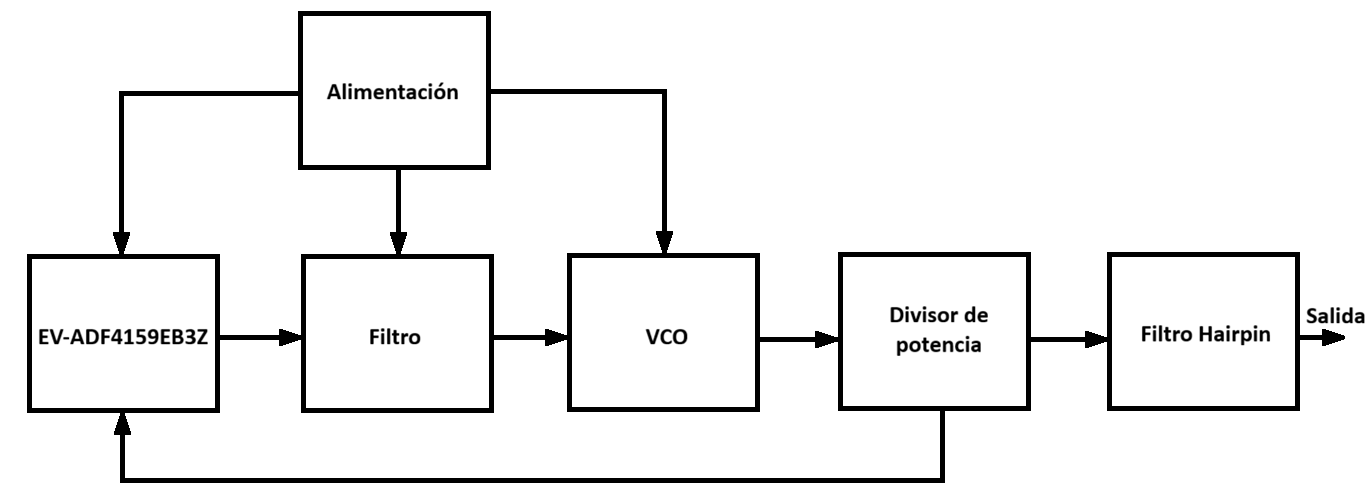
\includegraphics[width=0.95\textwidth]{imagenes/diagrama_sistema_completo.png}
    \caption{Diagrama en bloques del sistema completo. (Fuente: Propia).}
    \label{fig:diagrama_bloques_sistema_fmcw}
\end{figure}

La etapa de alimentación es la encargada de proporcionar las tensiones requeridas por los diferentes circuitos. La interfaz de usuario permite establecer los parámetros de funcionamiento del PLL, los cuales son enviados al dispositivo encargado de configurar el sintetizador de frecuencia.

El PLL recibe una señal de referencia y, a partir de los parámetros programados, genera la señal de control necesaria para el VCO. La salida del VCO es posteriormente distribuida mediante el divisor de potencia hacia las etapas correspondientes del sistema.

Esta arquitectura permite controlar tanto la frecuencia de salida como la evolución temporal de dicha frecuencia, posibilitando la generación de señales de frecuencia fija y de señales moduladas.

\section{Interfaz de usuario}

Para facilitar la configuración y operación del sistema se utilizó una interfaz de usuario proporcionada por Analog Devices que permite establecer los parámetros de funcionamiento del PLL modificando los registros del sintetizador.

La interfaz permite seleccionar la frecuencia de operación y configurar los parámetros asociados a la generación de la señal, tal como se muestra en la Figura~\ref{fig:interfaz_usuario}.

\begin{figure}[H]
    \centering
    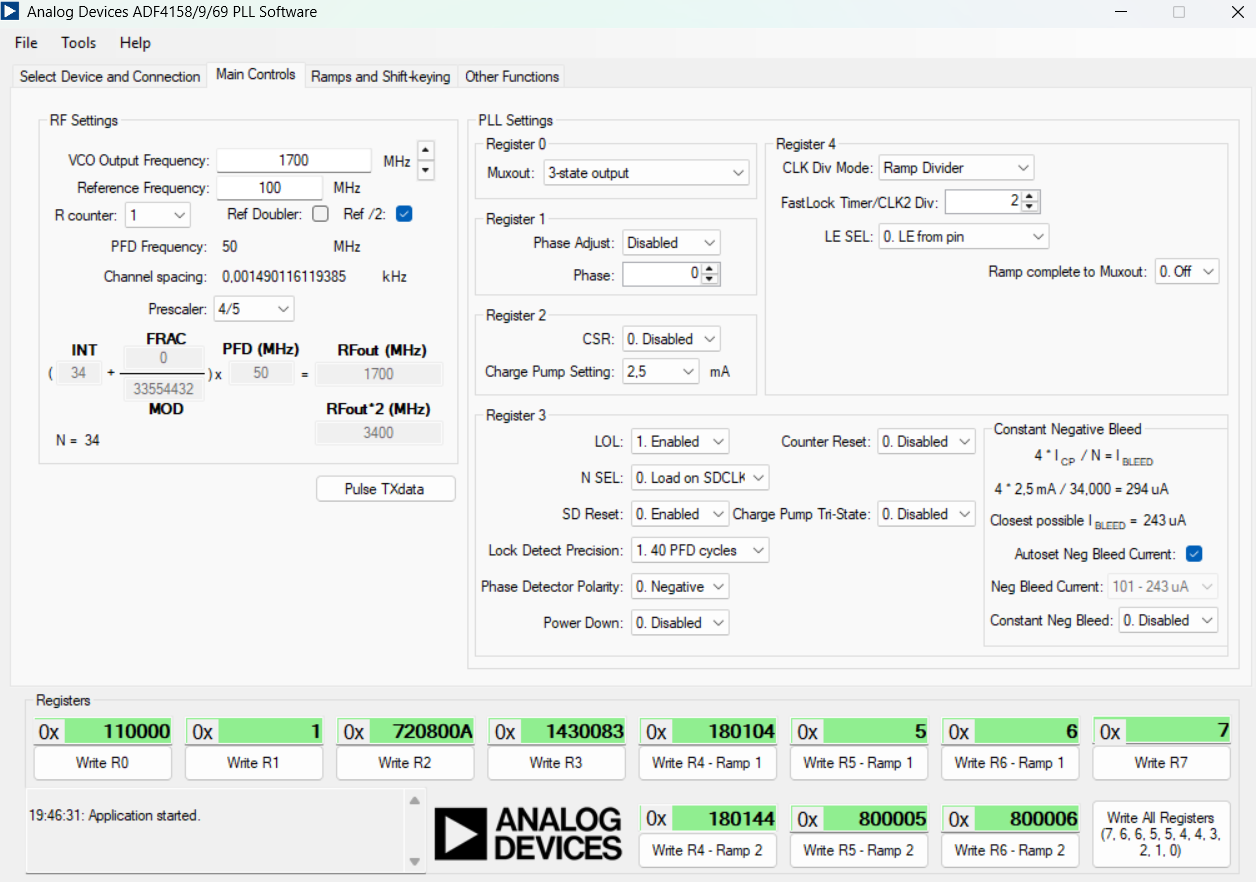
\includegraphics[width=0.85\textwidth]{imagenes/interfaz_usuario.png}
    \caption{Interfaz de usuario desarrollada para la configuración del sistema. (Fuente: Propia).}
    \label{fig:interfaz_usuario}
\end{figure}

\textbf{Main Controls:}
\begin{itemize}
    \item \textbf{VCO Output Frequency:} Frecuencia de salida del oscilador controlado por voltaje (VCO).
    
    \item \textbf{Reference Frequency:} Frecuencia de referencia externa proveniente de un oscilador presente en la placa EV-ADF4159EB3Z.
    
    \item \textbf{R counter:} Divisor de la frecuencia de referencia ($R$). Reduce la frecuencia de referencia antes de llegar al comparador de fase y frecuencia (PFD).
    
    \item \textbf{Ref Doubler:} Multiplicador por dos de la frecuencia de referencia de entrada.
    
    \item \textbf{Ref /2 (Marcado / Habilitado):} Divisor por dos de la frecuencia de referencia.
    
    \item \textbf{PFD Frequency:} Frecuencia del detector de fase ($f_{\mathrm{PFD}}$).
    
    \item \textbf{Channel spacing:} Espaciamiento entre canales o resolución del sintetizador de frecuencia.
    
    \item \textbf{Prescaler (4/5):} Predivisor dual de alta velocidad ubicado antes de los contadores enteros del lazo principal. Divide la frecuencia del VCO por 4 o por 5 bajo el control del módulo de control de pulsos.
    
    \item \textbf{INT:} Parte entera del divisor de realimentación del lazo de fase ($N$). Determina el múltiplo entero de la frecuencia del PFD.
    
    \item \textbf{FRAC:} Parte fraccional del divisor de realimentación. Permite un ajuste fino de la frecuencia entre canales enteros mediante modulación Sigma-Delta.
    
    \item \textbf{MOD:} Módulo de la sección fraccional (Sigma-Delta). Define el denominador de la fracción para el cálculo del canal y la resolución.
    
    \item \textbf{RFout:} Frecuencia de salida del divisor o del VCO.
    
    \item \textbf{RFout *2:} Frecuencia de salida duplicada.
    
    \item \textbf{Muxout:} Configuración del pin multiplexor de salida del circuito integrado.
    
    \item \textbf{Phase Adjust:} Control de ajuste de fase. Permite deshabilitar o habilitar el desplazamiento de fase programable de la salida.
    
    \item \textbf{Phase:} Valor de desfase programado en grados o radianes cuando el ajuste de fase está activo.
    
    \item \textbf{CSR (Cycle Slip Reduction):} Reducción de deslizamiento de ciclos.
    
    \item \textbf{Charge Pump Setting:} Corriente de la bomba de carga. Define la ganancia de la bomba de carga ($I_{\mathrm{CP}}$), parámetro crítico para la estabilidad y el ancho de banda del lazo de control.
    
    \item \textbf{CLK Div Mode:} Modo de división de reloj para funciones especiales de rampa o modulación de frecuencia.
    
    \item \textbf{FastLock Timer/CLK2 Div:} Reloj secundario para acelerar el tiempo de enganche (\textit{lock time}) del sintetizador.
    
    \item \textbf{LE SEL:} Configuración de la línea \textit{Latch Enable}, seleccionada para ser controlada directamente desde el pin físico del circuito integrado.
    
    \item \textbf{Ramp complete to Muxout:} Envía la señal indicadora de finalización de rampa hacia el pin Muxout.
    
    \item \textbf{LOL:} Detección de pérdida de enganche (\textit{Loss of Lock}).
    
    \item \textbf{N SEL:} Configuración de carga del registro $N$.
    
    \item \textbf{SD Reset:} Reinicio automático o manual del modulador Sigma-Delta para evitar estados estancados.
    
    \item \textbf{Charge Pump Tri-State:} Coloca la salida de la bomba de carga en alta impedancia (triestado).
    
    \item \textbf{Lock Detect Precision:} Precisión del detector de bloqueo. Requiere 40 ciclos consecutivos coincidentes del PFD para declarar que el lazo está enganchado.
    
    \item \textbf{Phase Detector Polarity:} Polaridad del detector de fase y frecuencia, configurada acorde a las características de ganancia del VCO y del filtro activo utilizados.
    
    \item \textbf{Power Down:} Modo de apagado o bajo consumo de energía del circuito integrado.
    
    \item \textbf{Constant Negative Bleed / I\_BLEED:} Corriente de sangrado constante negativa aplicada en la bomba de carga para mitigar la zona muerta.
\end{itemize}

La interfaz permite seleccionar además barridos de frecuencia y otros tipos de modulaciones, tal como se observa en la Figura~\ref{fig:interfaz_modulaciones}.

\begin{figure}[H]
    \centering
    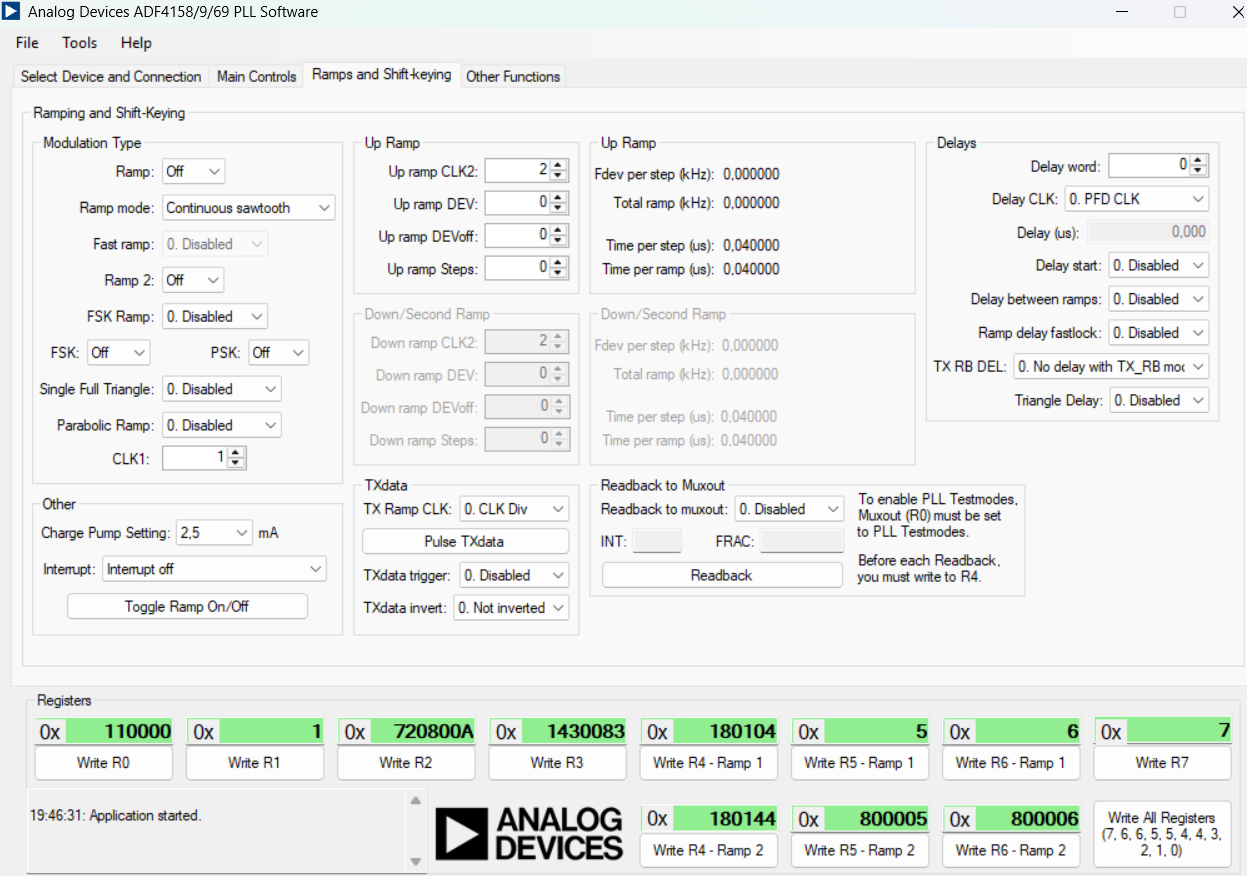
\includegraphics[width=0.85\linewidth]{imagenes/interfaz_modulaciones.png}
    \caption{Interfaz de usuario para la configuración de modulaciones. (Fuente: Propia).}
    \label{fig:interfaz_modulaciones}
\end{figure}

\begin{itemize}
    \item \textbf{Modulation Type - Ramp:} Habilita o deshabilita la función de generación de rampas de frecuencia.
    
    \item \textbf{Modulation Type - Ramp mode:} Define el modo de funcionamiento de la rampa (continua, disparo único, etc.).
    
    \item \textbf{Modulation Type - Fast ramp:} Habilita el modo de rampa rápida para transiciones aceleradas de frecuencia minimizando el sobrepasamiento.
    
    \item \textbf{Modulation Type - Ramp 2:} Controla la activación de un segundo perfil o conjunto de parámetros para una rampa alternativa.
    
    \item \textbf{Modulation Type - FSK:} Activa la modulación por desplazamiento de frecuencia (FSK).
    
    \item \textbf{Modulation Type - PSK:} Activa la modulación por desplazamiento de fase (PSK).
    
    \item \textbf{Modulation Type - Single Full Triangle:} Generación de un único ciclo completo de rampa triangular.
    
    \item \textbf{Modulation Type - Parabolic Ramp:} Habilita perfiles de rampa parabólica.
    
    \item \textbf{Modulation Type - CLK1:} Divisor del reloj base primario utilizado para temporizar la lógica de modulación y las rampas.
    
    \item \textbf{Other - Charge Pump Setting:} Configuración de la corriente de la bomba de carga durante la modulación.
    
    \item \textbf{Other - Interrupt:} Configuración de interrupciones por hardware para eventos relacionados con las rampas.
    
    \item \textbf{Up Ramp - Up ramp CLK2:} Divisor de reloj secundario que determina la base temporal durante la fase ascendente.
    
    \item \textbf{Up Ramp - Up ramp DEV:} Desviación de frecuencia o tamaño de paso programado en el registro.
    
    \item \textbf{Up Ramp - Up ramp DEVoff:} Desplazamiento o compensación en la desviación de frecuencia.
    
    \item \textbf{Up Ramp - Up ramp Steps:} Número total de pasos en la rampa ascendente.
    
    \item \textbf{Up Ramp - Fdev per step:} Desviación de frecuencia calculada para cada paso ascendente.
    
    \item \textbf{Up Ramp - Total ramp:} Desviación de frecuencia total durante toda la rampa ascendente.
    
    \item \textbf{Up Ramp - Time per step:} Duración temporal individual de cada paso.
    
    \item \textbf{Up Ramp - Time per ramp:} Tiempo total de duración de la rampa ascendente.
    
    \item \textbf{Down/Second Ramp:} Parámetros equivalentes configurados para la fase descendente o para el segundo perfil de rampa.
    
    \item \textbf{TXdata - TX Ramp CLK:} Selección de la fuente de reloj para la sincronización de las rampas en la transmisión de datos.
    
    \item \textbf{TXdata - TXdata trigger:} Señal de disparo para iniciar la transmisión de datos modulados por rampa.
    
    \item \textbf{TXdata - TXdata invert:} Invierte o mantiene la polaridad de los datos modulados transmitidos.
    
    \item \textbf{Readback to Muxout - Readback to muxout:} Permite leer registros internos del circuito integrado enviando su contenido a través del pin Muxout.
    
    \item \textbf{Delays - Delay word:} Registro para definir retardos temporales.
    
    \item \textbf{Delays - Delay CLK:} Selección de la base de tiempo o reloj utilizada para cuantificar los retardos.
    
    \item \textbf{Delays - Delay:} Tiempo absoluto de retardo programado.
    
    \item \textbf{Delays - Delay start:} Habilita un retardo inicial antes de que comience el proceso de modulación.
    
    \item \textbf{Delays - Delay between ramps:} Define un tiempo de pausa o espera entre la finalización de una rampa y el inicio de la siguiente.
    
    \item \textbf{Delays - Ramp delay fastlock:} Aplica un retardo controlado para acelerar el mecanismo de bloqueo rápido entre transiciones de rampa.
    
    \item \textbf{Delays - TX RB DEL:} Configura el retardo específico para los modos de lectura y retrocompatibilidad de transmisión.
    
    \item \textbf{Delays - Triangle Delay:} Añade un tiempo de retardo en los vértices de inversión de una rampa triangular.
\end{itemize}

\section{Cálculo de parámetros para la rampa FMCW}
A partir de las especificaciones requeridas (ancho de banda de $300~\mathrm{MHz}$, duración de $0{,}5~\mathrm{ms}$, frecuencia inicial de $1{,}55~\mathrm{GHz}$ y $f_{\mathrm{PFD}} = 50~\mathrm{MHz}$), se realizan los cálculos correspondientes para la configuración del ADF4159:

\subsection*{1. Resolución de frecuencia ($f_{\mathrm{RES}}$)}
\begin{equation}
f_{\mathrm{RES}} = \frac{f_{\mathrm{PFD}}}{2^{25}} = \frac{50~\mathrm{MHz}}{2^{25}} \approx 1{,}4901~\mathrm{Hz}.
\end{equation}

\subsection*{2. Desviación de frecuencia por paso ($f_{\mathrm{DEV}}$)}
Con un rango total de $300~\mathrm{MHz}$ distribuido en $1000$ pasos:
\begin{equation}
f_{\mathrm{DEV}} = \frac{300~\mathrm{MHz}}{1000} = 300~\mathrm{kHz}.
\end{equation}

\subsection*{3. Cálculo de $\mathrm{DEV\_OFFSET}$ y la palabra $\mathrm{DEV}$}
Empleando la ecuación de desplazamiento con $\mathrm{DEV}_{\max} = 2^{15} = 32768$ y fijando $\mathrm{DEV\_OFFSET} = 3$:
\begin{equation}
\mathrm{DEV} = \frac{f_{\mathrm{DEV}}}{f_{\mathrm{RES}} \times 2^{\mathrm{DEV\_OFFSET}}} = \frac{300~\mathrm{kHz}}{1{,}4901~\mathrm{Hz} \times 2^3} \approx 25165{,}82.
\end{equation}
Redondeando al entero más cercano para la programación del registro:
\begin{equation}
\mathrm{DEV} = 25166.
\end{equation}
Recalculando el ancho de banda y la desviación real obtenida:
\begin{equation}
f_{\mathrm{DEV\_real}} = 1{,}4901~\mathrm{Hz} \times 25166 \times 2^3 \approx 300{,}002~\mathrm{kHz},
\end{equation}
\begin{equation}
\text{Ancho de banda real} = 1000 \times 300{,}002~\mathrm{kHz} = 300{,}002~\mathrm{MHz}.
\end{equation}

\subsection*{4. Cálculo del temporizador ($\mathrm{CLK1}$ y $\mathrm{CLK2}$)}
Para cubrir el tiempo exacto de barrido de $0{,}5~\mathrm{ms}$ ($500~\mu\mathrm{s}$) en $1000$ pasos, el tiempo asignado a cada paso resulta de $0{,}5~\mu\mathrm{s}$. Fijando $\mathrm{CLK1} = 1$:
\begin{equation}
\mathrm{CLK2} = 0{,}5~\mu\mathrm{s} \times 50~\mathrm{MHz} = 25.
\end{equation}

\subsection*{Resumen de configuración adoptada}
\begin{itemize}
    \item \textbf{DEV:} $25166$
    \item \textbf{DEV\_OFFSET:} $3$
    \item \textbf{Número de pasos:} $1000$
    \item \textbf{CLK2:} $25$
    \item \textbf{CLK1:} $1$
    \item \textbf{Tiempo total de barrido:} $0{,}5~\mathrm{ms}$
    \item \textbf{Ancho de banda real:} $300{,}002~\mathrm{MHz}$ 
    \item \textbf{Frecuencia central:} $1{,}70~\mathrm{GHz}$ (barrido de $1{,}55~\mathrm{GHz}$ a $1{,}85~\mathrm{GHz}$)
\end{itemize}

En la Tabla~\ref{tab:fmcw_params} se resume la configuración de parámetros requerida para obtener diferentes tiempos de rampa en el sintetizador.

\begin{table}[H]
\centering
\resizebox{\textwidth}{!}{%
\begin{tabular}{lcccccc}
\toprule
\textbf{Tiempo de barrido} & \textbf{Pasos ($N$)} & \textbf{DEV} & \textbf{DEV\_OFFSET} & \textbf{CLK2} & \textbf{CLK1} & \textbf{BW Real (MHz)} \\
\midrule
$1~\mathrm{ms}$     & $1000$ & $25166$ & $3$ & $50$ & $1$ & $300{,}002$ \\
$0{,}5~\mathrm{ms}$   & $1000$ & $25166$ & $3$ & $25$ & $1$ & $300{,}002$ \\
$0{,}25~\mathrm{ms}$ & $1250$ & $20133$ & $3$ & $10$ & $1$ & $300{,}005$ \\
$0{,}05~\mathrm{ms}$ & $1250$ & $20133$ & $3$ & $2$  & $1$ & $300{,}005$ \\
$0{,}02~\mathrm{ms}$ & $500$  & $25166$ & $4$ & $2$  & $1$ & $300{,}002$ \\
\bottomrule
\end{tabular}%
}
\caption{Configuración de parámetros del ADF4159 para diferentes tiempos de barrido ($BW = 300~\mathrm{MHz}$, $f_{\mathrm{PFD}} = 50~\mathrm{MHz}$).}
\label{tab:fmcw_params}
\end{table}

\section{Simulación de la modulación en ADIsimPLL}

Antes de realizar la implementación experimental, se verificó el comportamiento de la modulación mediante el software ADIsimPLL, tal como se observa en la Figura~\ref{fig:adisimpll_modulacion}. Esta herramienta permite modelar el funcionamiento del sintetizador y analizar la respuesta del PLL ante diferentes configuraciones de frecuencia y parámetros de rampa.

\begin{figure}[H]
    \centering
    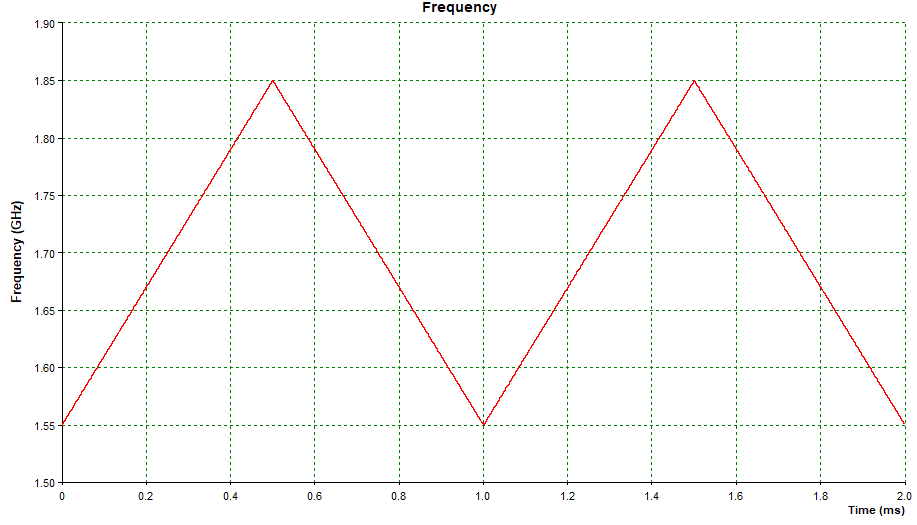
\includegraphics[width=0.75\textwidth]{imagenes/simulaciones_adisim.png}
    \caption{Simulación de la modulación de frecuencia del PLL mediante ADIsimPLL. (Fuente: Propia).}
    \label{fig:adisimpll_modulacion}
\end{figure}

A partir de los resultados obtenidos se verificó que el PLL es capaz de seguir la modulación configurada, manteniendo el control de la frecuencia de salida durante el intervalo de operación.

\section{Medición}

Se realizaron las mediciones del sistema configurando la rampa de frecuencia en modo triangular para un ancho de banda total de $300~\mathrm{MHz}$ ($1{,}55~\mathrm{GHz}$ a $1{,}85~\mathrm{GHz}$). Las pruebas se llevaron a cabo evaluando los mismos tiempos de barrido analizados en la etapa de diseño y simulación: $1~\mathrm{ms}$, $0{,}5~\mathrm{ms}$, $0{,}25~\mathrm{ms}$, $0{,}05~\mathrm{ms}$ y $0{,}02~\mathrm{ms}$, utilizando los parámetros de configuración previamente calculados. A continuación se presentan las mediciones correspondientes a los casos de $1~\mathrm{ms}$ y $0{,}02~\mathrm{ms}$.

\subsection{Respuesta en frecuencia (Analizador de espectro)}
Para verificar el funcionamiento del sistema bajo los extremos de velocidad evaluados, se registró la envolvente del \textit{chirp} triangular en el analizador de espectro.

La Figura~\ref{fig:chirp_mayor} muestra la medición correspondiente al mayor tiempo de barrido ($1~\mathrm{ms}$), donde se observa la máxima estabilidad y resolución temporal del barrido de frecuencia. Por otro lado, la Figura~\ref{fig:chirp_menor} muestra el resultado para el menor tiempo de barrido ($0{,}02~\mathrm{ms}$ o $20~\mu\mathrm{s}$), evidenciando que la velocidad de conmutación excede la capacidad de seguimiento del lazo de enganche de fase (PLL).

\begin{figure}[htbp]
    \centering
    \begin{subfigure}[b]{0.48\textwidth}
        \centering
        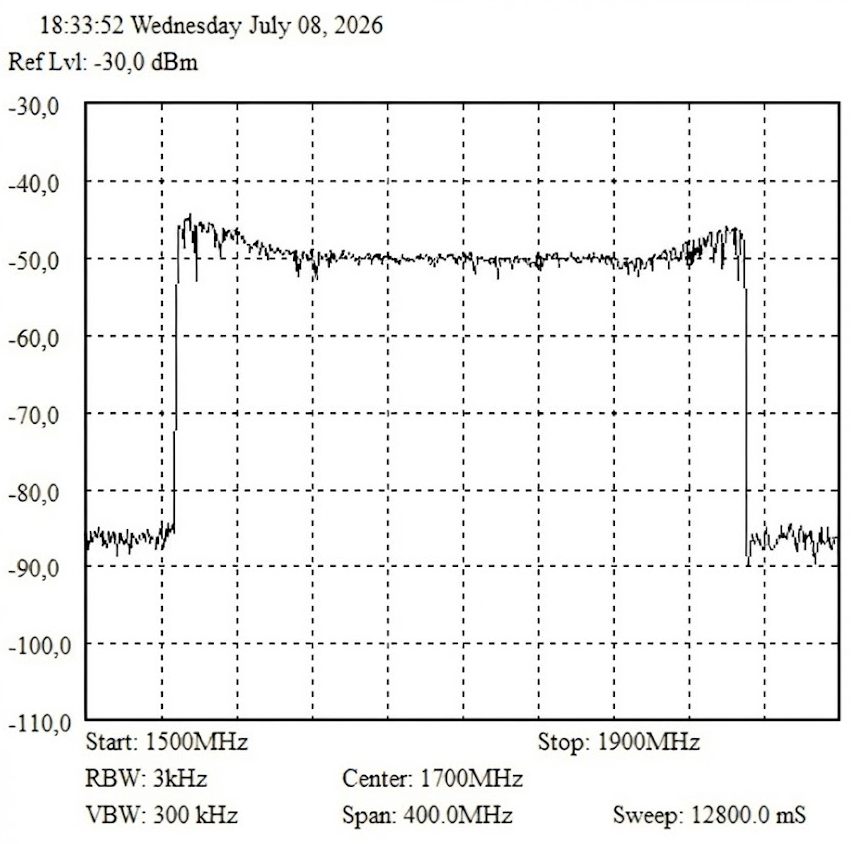
\includegraphics[width=\textwidth]{imagenes/chirp_1ms.png}
        \caption{Tiempo de barrido máximo ($T = 1~\mathrm{ms}$).}
        \label{fig:chirp_mayor}
    \end{subfigure}
    \hfill
    \begin{subfigure}[b]{0.48\textwidth}
        \centering
        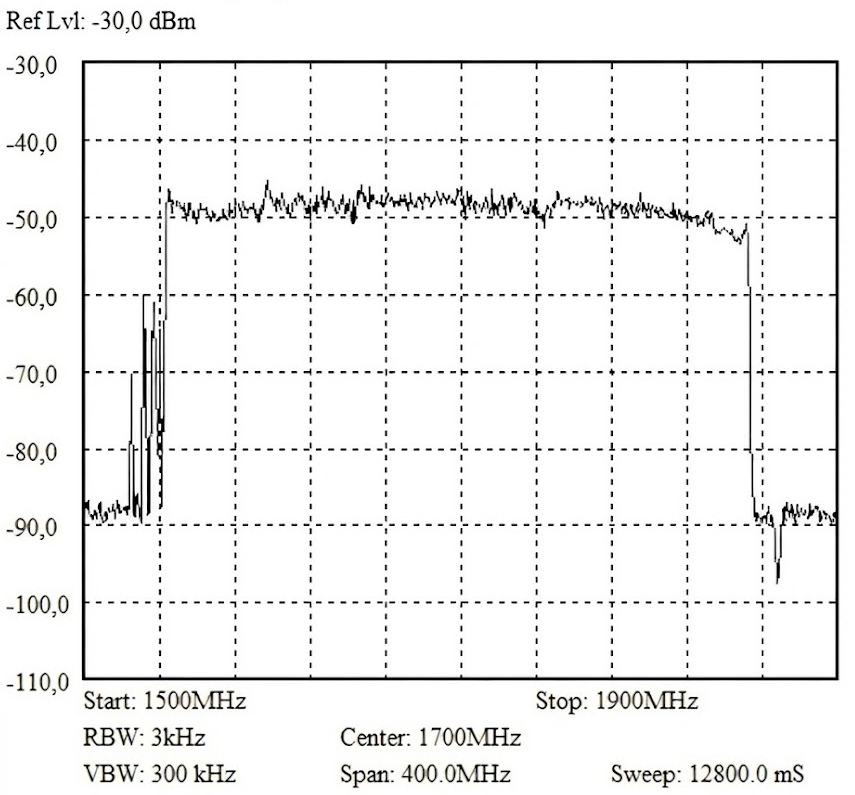
\includegraphics[width=\textwidth]{imagenes/chirp_002ms.png}
        \caption{Tiempo de barrido mínimo ($T = 0{,}02~\mathrm{ms}$).}
        \label{fig:chirp_menor}
    \end{subfigure}
    \caption{Chirps triangulares medidos en el analizador de espectro para los extremos de velocidad de barrido. (Fuente: Propia).}
    \label{fig:chirps_comparacion}
\end{figure}

La Figura~\ref{fig:chirp_sierra_mayor} muestra la medición correspondiente al mayor tiempo de barrido ($1~\mathrm{ms}$), donde se observa el comportamiento del \textit{chirp} diente de sierra a una velocidad reducida de variación de frecuencia. Por otro lado, la Figura~\ref{fig:chirp_sierra_menor} presenta el resultado obtenido para un tiempo de barrido de $0{,}25~\mathrm{ms}$, correspondiente a una mayor velocidad de variación de frecuencia. Mediciones con tiempos inferiores a $0{,}25~\mathrm{ms}$ presentan degradaciones apreciables en la linealidad del barrido.

\begin{figure}[H]
    \centering
    \begin{subfigure}[b]{0.48\textwidth}
        \centering
        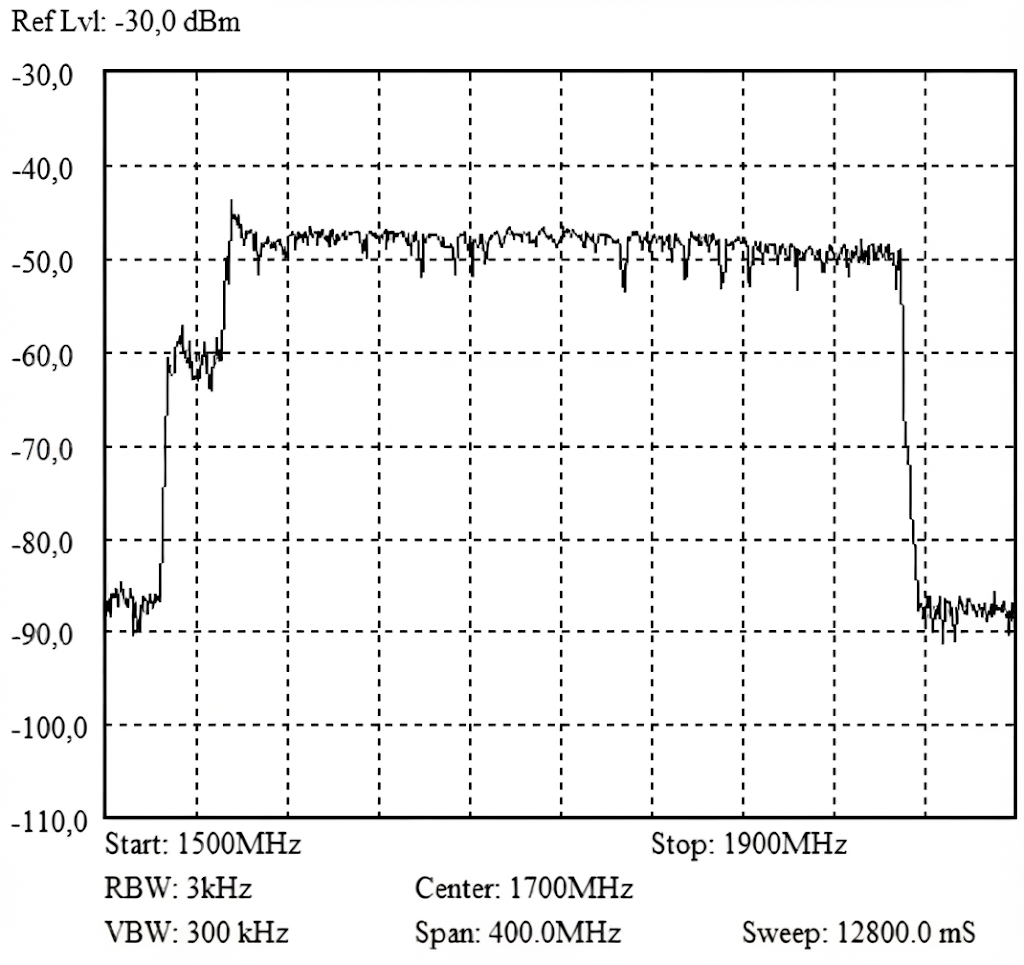
\includegraphics[width=\textwidth]{imagenes/chirp_sierra_1ms.png}
        \caption{Tiempo de barrido ($T = 1~\mathrm{ms}$).}
        \label{fig:chirp_sierra_mayor}
    \end{subfigure}
    \hfill
    \begin{subfigure}[b]{0.48\textwidth}
        \centering
        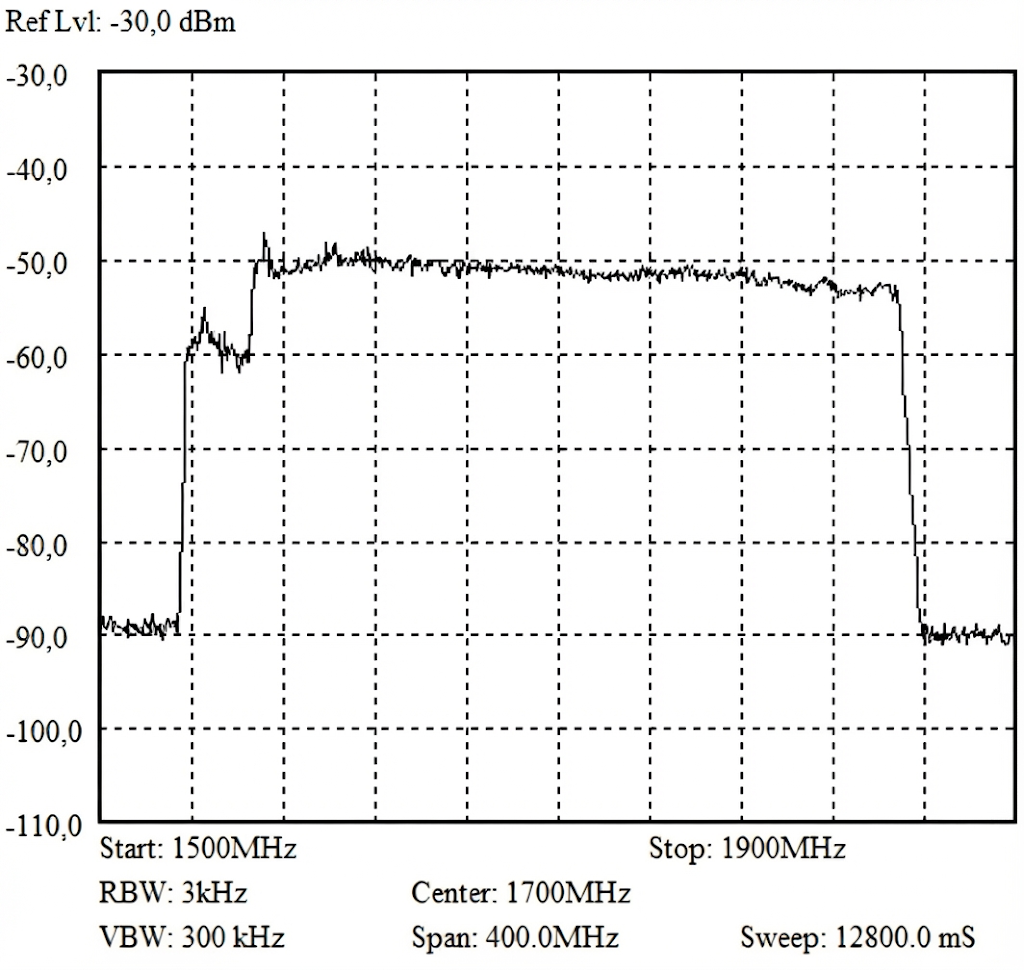
\includegraphics[width=\textwidth]{imagenes/chirp_sierra_025ms.png}
        \caption{Tiempo de barrido ($T = 0{,}25~\mathrm{ms}$).}
        \label{fig:chirp_sierra_menor}
    \end{subfigure}
    \caption{Chirps de tipo diente de sierra medidos en el analizador de espectro para dos tiempos de barrido. (Fuente: Propia).}
    \label{fig:chirps_sierra_comparacion}
\end{figure}

En la Figura~\ref{fig:chirp_sierra_menor} se observa una reducción en el nivel de potencia sobre el extremo inferior de frecuencia del barrido, originada por el sobrepasamiento transitorio de la tensión de sintonía al reiniciarse la rampa.

\subsection{Tensiones de control (Osciloscopio)}
Con el fin de analizar el comportamiento dinámico del sistema y comprobar la linealidad de la rampa, se midieron las formas de onda de la tensión de control en el nodo de sintonía utilizando un osciloscopio.

En la Figura~\ref{fig:tensiones_control} se presentan las tensiones de control correspondientes a los extremos temporales evaluados para el modo triangular ($1~\mathrm{ms}$ y $0{,}02~\mathrm{ms}$).

\begin{figure}[H]
    \centering
    \begin{subfigure}[b]{0.48\textwidth}
        \centering
        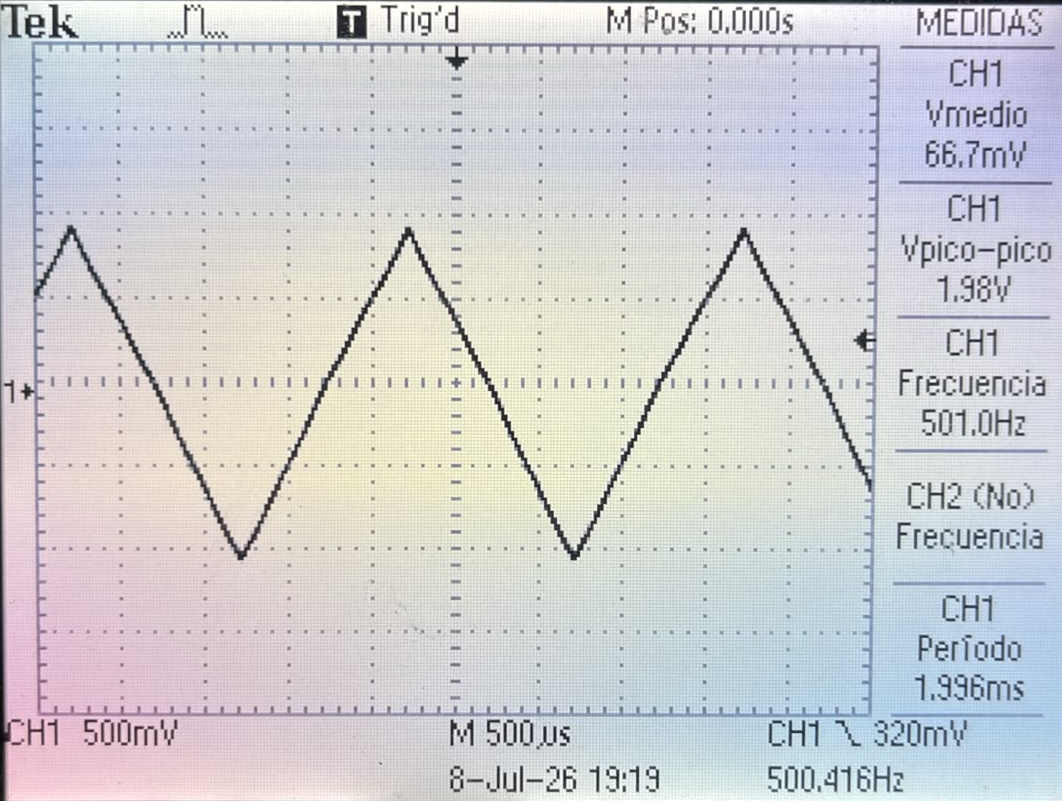
\includegraphics[width=\textwidth]{imagenes/tension_control1ms.png}
        \caption{Tensión de control para $T = 1~\mathrm{ms}$.}
        \label{fig:tension_1ms}
    \end{subfigure}
    \hfill
    \begin{subfigure}[b]{0.48\textwidth}
        \centering
        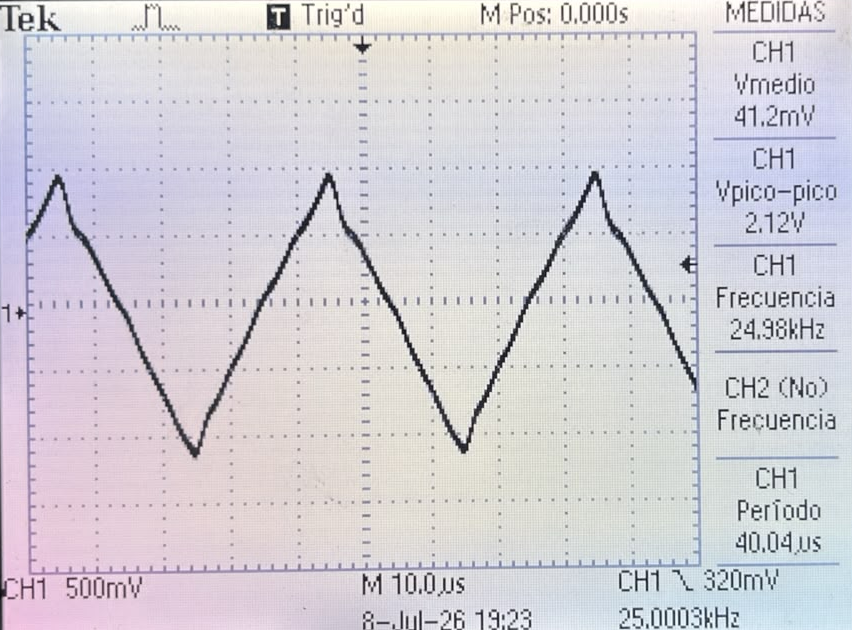
\includegraphics[width=\textwidth]{imagenes/tension_control002ms.png}
        \caption{Tensión de control para $T = 0{,}02~\mathrm{ms}$.}
        \label{fig:tension_002ms}
    \end{subfigure}
    \caption{Formas de onda de la tensión de control medidas en el osciloscopio para los tiempos de barrido de $1~\mathrm{ms}$ y $0{,}02~\mathrm{ms}$. (Fuente: Propia).}
    \label{fig:tensiones_control}
\end{figure}

En la Figura~\ref{fig:tensiones_control_sierra} se presentan las formas de onda de la tensión de control correspondientes a los dos tiempos de barrido evaluados para el \textit{chirp} de tipo diente de sierra ($1~\mathrm{ms}$ y $0{,}25~\mathrm{ms}$).

\begin{figure}[H]
    \centering
    \begin{subfigure}[b]{0.48\textwidth}
        \centering
        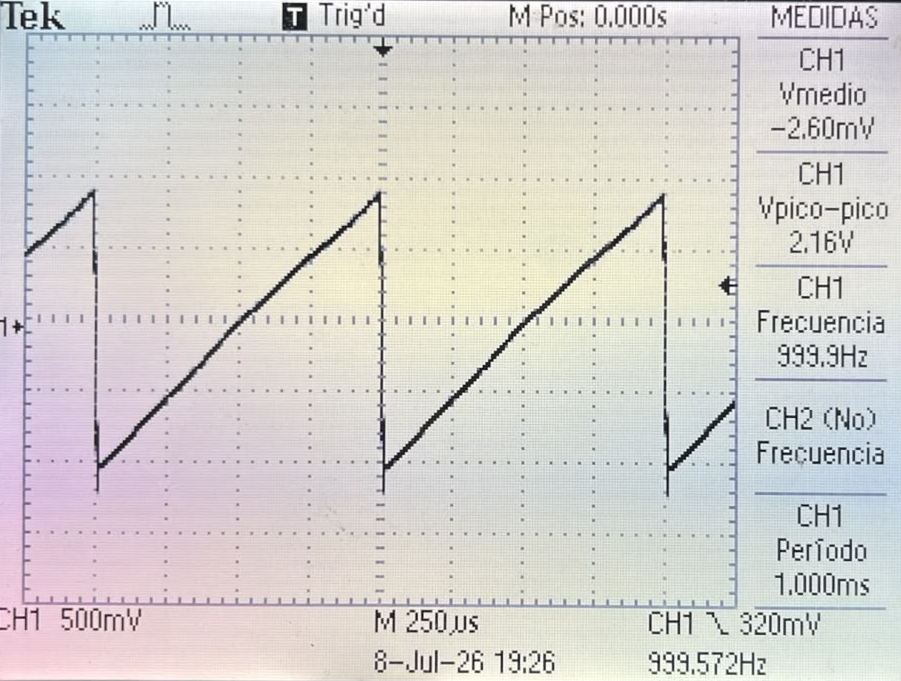
\includegraphics[width=\textwidth]{imagenes/tension_control_sierra1ms.png}
        \caption{Tensión de control para $T = 1~\mathrm{ms}$.}
        \label{fig:tension_sierra_1ms}
    \end{subfigure}
    \hfill
    \begin{subfigure}[b]{0.48\textwidth}
        \centering
        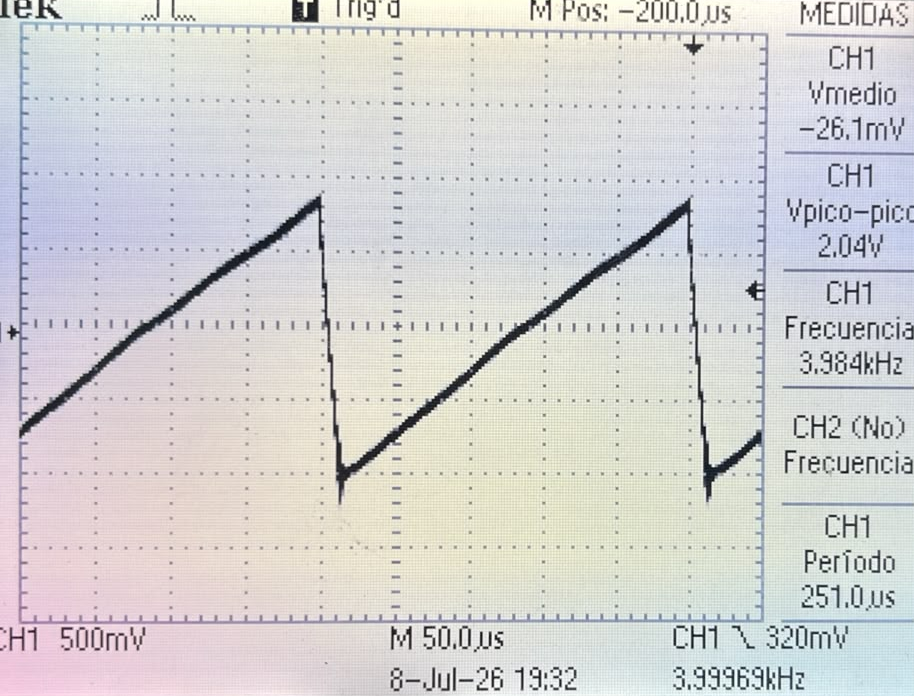
\includegraphics[width=\textwidth]{imagenes/tension_control_sierra025ms.png}
        \caption{Tensión de control para $T = 0{,}25~\mathrm{ms}$.}
        \label{fig:tension_sierra_025ms}
    \end{subfigure}
    \caption{Formas de onda de la tensión de control medidas en el osciloscopio para los tiempos de barrido de $1~\mathrm{ms}$ y $0{,}25~\mathrm{ms}$ del chirp diente de sierra. (Fuente: Propia).}
    \label{fig:tensiones_control_sierra}
\end{figure}

A partir de las mediciones se observa que el sobrepasamiento transitorio se incrementa de forma apreciable a medida que el período de barrido se reduce.

\subsection{Comparación de rampas}
Finalmente, se realizó una comparación directa entre las rampas de frecuencia generadas para diferentes tiempos de barrido ($0{,}5~\mathrm{ms}$, $0{,}05~\mathrm{ms}$ y $0{,}02~\mathrm{ms}$) y el comportamiento del VCO operando a lazo abierto. Esta comparación permite evaluar el desempeño del sistema al incrementar progresivamente la velocidad de modulación y determinar los límites prácticos de seguimiento del PLL.

La Figura~\ref{fig:comparacion_rampas} presenta las rampas obtenidas. A medida que se reduce el tiempo de barrido, aumenta la pendiente de la rampa de frecuencia, exigiendo una mayor velocidad de respuesta al lazo cerrado. De esta manera, el ensayo permite verificar experimentalmente el margen de estabilidad y el seguimiento dinámico del sistema ante diferentes velocidades de modulación.

\begin{figure}[H]
    \centering
    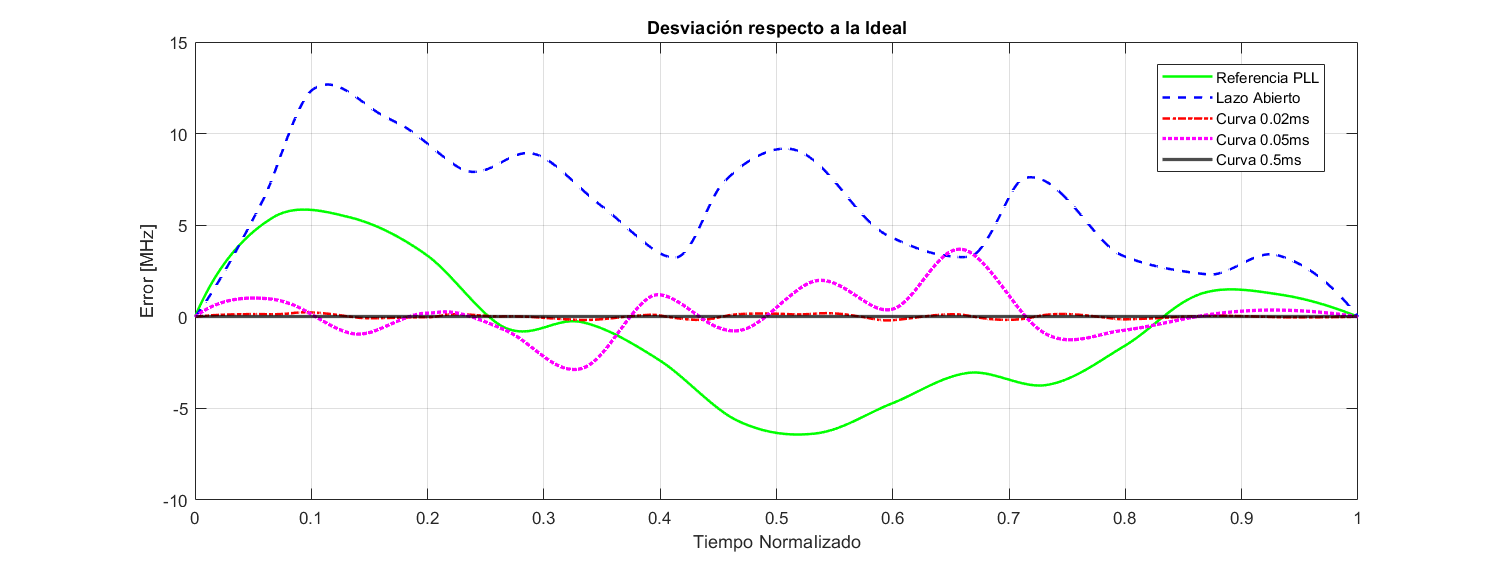
\includegraphics[width=0.95\textwidth]{imagenes/comparaciónrampas.png}
    \caption{Comparación de las rampas de frecuencia generadas para tiempos de barrido de $0{,}5~\mathrm{ms}$, $0{,}05~\mathrm{ms}$ y $0{,}02~\mathrm{ms}$. (Fuente: Propia).}
    \label{fig:comparacion_rampas}
\end{figure}

En la rampa de $0{,}5~\mathrm{ms}$ el PLL consigue seguir adecuadamente la modulación impuesta por el sintetizador, registrando una desviación de frecuencia máxima de tan solo $240~\mathrm{kHz}$ respecto al perfil ideal. 

Sin embargo, al incrementar la velocidad de modulación reduciendo el tiempo de barrido a $0{,}05~\mathrm{ms}$, la inercia dinámica del lazo y los retardos del sistema se vuelven más patentes, elevándose la desviación de frecuencia máxima hasta los $2{,}5~\mathrm{MHz}$. 

Finalmente, para el caso extremo de la rampa de $0{,}02~\mathrm{ms}$, el análisis temporal revela un comportamiento particular: al evaluar de forma aislada un único período de la onda, la traza de la rampa del VCO a lazo abierto aparenta una mayor linealidad. No obstante, esta aparente ventaja del modo libre es efímera y limitada, ya que no contempla la falta de repetitividad temporal inherente al oscilador sin control de fase. Mientras que el PLL, a pesar de sus limitaciones transitorias en frecuencias de conmutación muy elevadas, garantiza la estabilidad a largo plazo y la sincronización estricta entre ciclos consecutivos, el VCO a lazo abierto deriva térmicamente y carece de la repetitividad indispensable para el procesamiento coherente de señales en un radar FMCW.

\subsection{Ruido de fase}

Se realizó la medición del ruido de fase del PLL configurado en una frecuencia fija dentro de la banda de interés, con el objetivo de caracterizar la estabilidad espectral de la señal generada por el sistema integrado. El resultado obtenido experimentalmente se presenta en la Figura~\ref{fig:ruido_fase_pll}.

\begin{figure}[H]
    \centering
    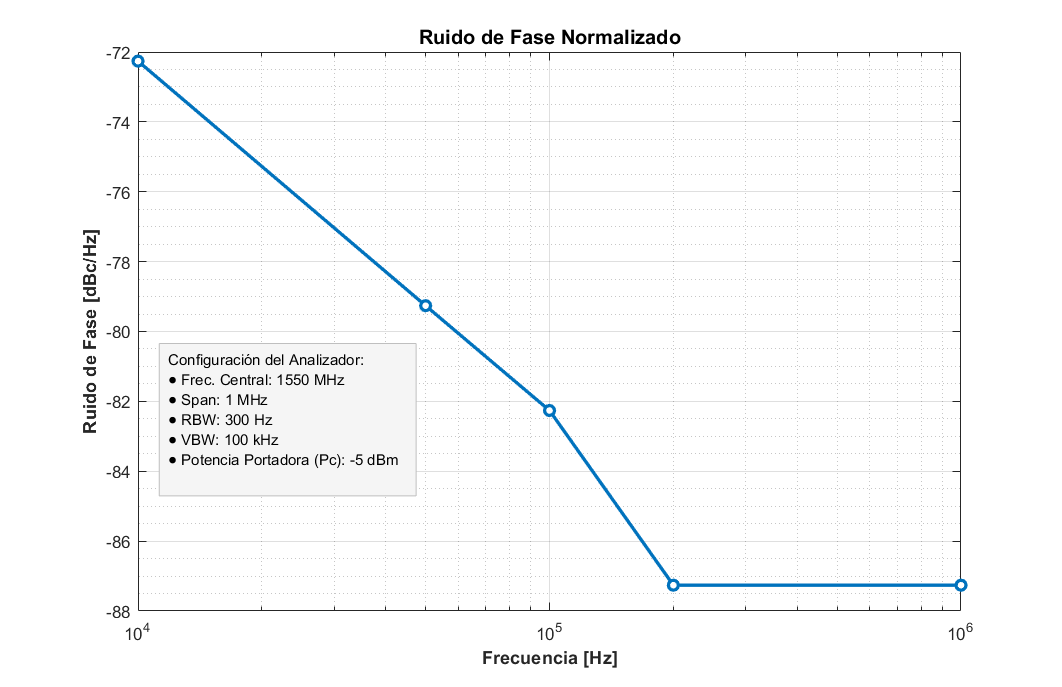
\includegraphics[width=0.85\textwidth]{imagenes/ruido_fase_pll.png}
    \caption{Medición del ruido de fase del PLL a frecuencia fija. (Fuente: Propia).}
    \label{fig:ruido_fase_pll}
\end{figure}

Teniendo en cuenta la medición previa del VCO en solitario, el ruido de fase del sistema integrado con el PLL disminuyó $7~\mathrm{dBc}$ en promedio para todas las frecuencias analizadas.